\documentclass[12pt]{extarticle}
\usepackage[utf8]{inputenc}
\usepackage[english]{babel}
\usepackage[utf8]{inputenc}
\usepackage[english]{babel}
\usepackage[a4paper, total={7in, 9.5in}]{geometry}
\usepackage{tikz-cd}

 
\usepackage{amsthm, amssymb, amsmath, centernot, graphicx}
\usepackage{accents}
\DeclareMathAccent{\wtilde}{\mathord}{largesymbols}{"65}
\newcommand{\orb}[1]{\mathrm{Orb}(#1)}
\newcommand{\stab}[1]{\mathrm{Stab}(#1)}
\newcommand{\rp}{\mathbb{RP}}
\newcommand{\cp}{\mathbb{CP}}

\newcommand{\notimplies}{%
  \mathrel{{\ooalign{\hidewidth$\not\phantom{=}$\hidewidth\cr$\implies$}}}}
 
\renewcommand\qedsymbol{$\square$}
\newcommand{\cont}{$\boxtimes$}
\newcommand{\divides}{\mid}
\newcommand{\ndivides}{\centernot \mid}
\newcommand{\Z}{\mathbb{Z}}
\newcommand{\N}{\mathbb{N}}
\newcommand{\C}{\mathbb{C}}
\newcommand{\Zplus}{\mathbb{Z}^{+}}
\newcommand{\Primes}{\mathbb{P}}
\newcommand{\ball}[2]{B_{#1} \! \left(#2 \right)}
\newcommand{\Q}{\mathbb{Q}}
\newcommand{\R}{\mathbb{R}}
\newcommand{\Rplus}{\mathbb{R}^+}
\newcommand{\invI}[2]{#1^{-1} \left( #2 \right)}
\newcommand{\End}[1]{\text{End}\left( A \right)}
\newcommand{\legsym}[2]{\left(\frac{#1}{#2} \right)}
\renewcommand{\mod}[3]{\: #1 \equiv #2 \: \mathrm{mod} \: #3 \:}
\newcommand{\nmod}[3]{\: #1 \centernot \equiv #2 \: mod \: #3 \:}
\newcommand{\ndiv}{\hspace{-4pt}\not \divides \hspace{2pt}}
\newcommand{\finfield}[1]{\mathbb{F}_{#1}}
\newcommand{\finunits}[1]{\mathbb{F}_{#1}^{\times}}
\newcommand{\ord}[1]{\mathrm{ord}\! \left(#1 \right)}
\newcommand{\quadfield}[1]{\Q \small(\sqrt{#1} \small)}
\newcommand{\vspan}[1]{\mathrm{span}\! \left\{#1 \right\}}
\newcommand{\galgroup}[1]{Gal \small(#1 \small)}
\newcommand{\sm}{\! \setminus \!}
\newcommand{\topo}{\mathcal{T}}
\newcommand{\base}{\mathcal{B}}
\renewcommand{\bf}[1]{\mathbf{#1}}
\renewcommand{\Im}[1]{\mathrm{Im} \: #1}
\renewcommand{\empty}{\varnothing}
\newcommand{\id}{\mathrm{id}}
\newcommand{\Hom}[2]{\mathrm{Hom}\left( #1, #2 \right)}
\newcommand{\Tor}[4]{\mathrm{Tor}^{#1}_{#2} \left( #3, #4 \right)}

\renewcommand{\theenumi}{(\alph{enumi})}

\newcommand{\atitle}[1]{\title{% 
	\large \textbf{Mathematics GU4053 Algebraic Topology
	\\ Assignment \# #1} \vspace{-2ex}}
\author{Benjamin Church }
\maketitle}

\newcommand{\hook}{\hookrightarrow}


\theoremstyle{remark}
\newtheorem*{remark}{Remark}

\theoremstyle{definition}
\newtheorem{theorem}{Theorem}[section]
\newtheorem{lemma}[theorem]{Lemma}
\newtheorem{proposition}[theorem]{Proposition}
\newtheorem{corollary}[theorem]{Corollary}
\newtheorem{example}[theorem]{Example}


\newenvironment{definition}[1][Definition:]{\begin{trivlist}
\item[\hskip \labelsep {\bfseries #1}]}{\end{trivlist}}

\usepackage{subcaption}
\usepackage{float}
\floatplacement{figure}{H}
\usepackage{tikz-feynman}
\tikzfeynmanset{compat=1.0.0} 


\begin{document}
\atitle{3}

Note. My order of path concatenation follows lectures,
\[\gamma * \delta(x) = \begin{cases}
\delta(2x) & x \le \tfrac{1}{2} \\
\gamma(2x - 1) & x \ge \tfrac{1}{2}
\end{cases}\]
 
\section*{Problem 1.}

Let $M_0 = \R^n$ for $n \ge 3$. Let $S \subset \R^n$ be finite. Take a finite sequence $s_i$ which exhausts $S$. Then define $M_{i} = M_{i - 1} \sm \{s_i\}$. Suppose that $M_{i - 1}$ is a simply-connected $n$-manifold. Then, by Lemma \ref{manifoldlessapoint}, $M_i$ is simply-connected. However, $M_i = \R^n \sm A$ for $A \subset S \subset \R^n$ finite so, by Lemma \ref{ismanifold}, $M_i$ is a simply-connected $n$-manifold. Also, $M_0 = \R^n$ is contractable and thus simply-connected. By induction, every $M_n$ is simply-connected. Therefore, $M_N = \R^n \sm S$ for $N = |S|$ is simply connected.   

\section*{Problem 2.}

Let $X \subset \R^3$ be a union of $n$ lines through the origin. First, consider $\R^3$ minus a single line which deformation retracts onto a hollow cylinder about the line. The next $n - 1$ lines each intersect the cylinder in exactly two points. Therefore, $\R^3 \sm X$ deformation retracts to a cylinder minus $2(n - 1)$ points which futher deformation retracts to a plane minus $2n - 1$ points (since a cylinder is homeomorphic to a punctured plane under the logarithm map). The plane minus $2n - 1$ points deformation retracts onto the wedge of $2n - 1$ circles. Thus, 
\[\pi_1(\R^3 \sm X) \cong \pi_1\left( \bigvee\limits_{i = 1}^{2n - 1} S^1 \right) \cong \Z^{(2n - 1)*} \] 

\section*{Problem 3.}

Let $A$ be an open set containing the first torus and a small section (not containing any nontrivial loops) of the second torus. Similarly, let $B$ be an open set containing the second torus and a small section of the first. Then, $X = A \cup B$. Because we did not contain any nontrivial loops in the other tori, we can deformation retract $A$ and $B$ onto a single torus. Thus, $\pi_1(A, x_0) \cong \Z \times \Z $ and $\pi_1(B, x_0) \cong \Z \times \Z$. However, the intersection $A \cap B$ is path-connected and deformation retracts to $S^1 \times \{x_0\}$ which is the circle identified in both tori. Therefore, $\pi_1(X, x_0) \cong (\Z \times \Z) * ( \Z \times \Z ) / \sim$ where $(n, 0)_1 \sim (n, 0)_2$ since the inclusion maps of $S^1 \times \{x_0\}$ into $A$ and $B$ will take a loop that goes arround $n$ times into the terms $(n, 0)_1$ and $(n, 0)_2$ which then must be equal. Denote $(n, 0)_1$ by $a^n$ and $b^n = (0, n)_1$ and $c^n = (0, n)_2$. Then, $ab = ba$ because,
\[(1, 0)_1 * (0, 1)_1 = (1, 0)_1 + (0, 1)_1 = (1, 1)_1 = (0, 1)_1 * (1, 0)_1\]
Likewise, $ac = ca$ because,
\[(1, 0)_1 * (0, 1)_2 = (1, 0)_2 * (0, 1)_2 = (1, 0)_2 + (0, 1)_2 = (1, 1)_2 = (0, 1)_2 * (1, 0)_2 = (0, 1)_2 * (1, 0)_1\]
Therefore,
\[ \pi_1(X, x_0) \cong \left< a, b, c \mid aba^{-1}b^{-1} = e, aca^{-1}c^{-1} = e \right> \]
This is more easily seen from the identification space,
\begin{center}
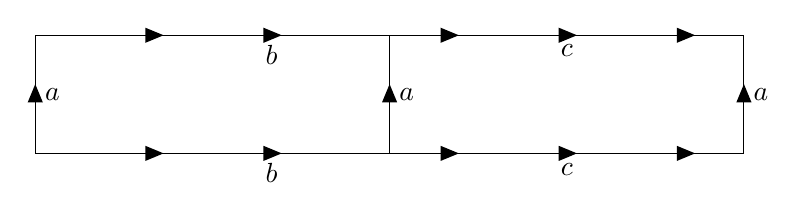
\begin{tikzpicture}
\begin{feynman}
\vertex (a) ;
\vertex [above =of a] (b) ;
\vertex [right =of b] (i1) ;
\vertex [right =of i1] (i2) ;
\vertex [right =of i2] (c) ;
\vertex [right =of c] (j1) ;
\vertex [right =of j1] (j2) ;
\vertex [right =of j2] (d) ;
\vertex [below =of d] (e) ;
\vertex [left =of e] (k1) ;
\vertex [left =of k1] (k2) ;
\vertex [left =of k2] (f) ;
\vertex [right =of a] (l1) ;
\vertex [right =of l1] (l2) ;

\diagram* {
(a) -- [fermion,  edge label'= \(a\)] (b),
(b) -- [fermion] (i2),
(i1) -- [fermion,  edge label'= \(b\)] (c),
(c) -- [fermion] (j1),
(j1) -- [fermion,  edge label'= \(c\)] (j2),
(j2) -- [fermion] (d),
(e) -- [fermion,  edge label'= \(a\)] (d),
(f) -- [fermion] (k2),
(k2) -- [fermion,  edge label'= \(c\)] (k1),
(k1) -- [fermion] (e),
(f) -- [fermion,  edge label'= \(a\)] (c),
(a) -- [fermion] (l2),
(l1) -- [fermion,  edge label'= \(b\)] (f),

};
\end{feynman}
\end{tikzpicture} 
\end{center}
In which the relations $aba^{-1}b^{-1} = e$ and $aca^{-1}c^{-1} = e$ are obvious  by contracting the squares.  
\section*{Problem 4.}

Let $X = \R^2 \sm \Q^2$. Take your favorite irrational number $x_0 \in \R \sm \Q$. Take any $x \in \R \sm \Q$ then consider the square defined by the coordinates, $(x_0, x_0), (x_0, x), (x, x_0), (x, x)$. The boundary of this square has no points in $\Q^2$ because $x, x_0 \notin \Q$ so traversing this boundard defines a loop $\gamma_x : I \to X$ at $(x_0, x_0)$. I claim that if $x \neq y$ for $x, y \in \R \sm \Q$ then $\gamma_x$ and $\gamma_y$ are not homotopic. Without loss of generality, take $x < y$ so there exists $q \in [x, y] \cap \Q$. Because $X \subset \R^2 \sm \{(q, q)\}$ if the paths $\gamma_x$ and $\gamma_y$ are homotopic in $X$ then they must also be homotopic in $\R^2 \sm \{(q, q)\}$. However, $(q, q)$ is in the interior of $\gamma_y$ but not of $\gamma_x$ so $\gamma_x$ is homotopic to the constant path but $\gamma_y$ cannot be because it must generate the fundamental group. However, the punctured plane retracts onto the circle so it has a nontrivial fundamental group. Therefore, $\gamma_x$ and $\gamma_y$ are not homotopic in $\R^2 \sm \{(q, q)\}$ and thus not homotopic in $X$ thus proving the claim. Therefore, there is an injection from $\R$ into homotopy classes of loops at $(x_0, x_0)$ in $X$. Thus, $\pi_1(\R^2 \sm \Q^2, (x_0, x_0))$ is uncountable. 

\section*{Problem 5.}
Are the following categories?
\begin{enumerate}
\item Objects are finite sets, morphisms are injective maps of sets: \bigskip\\
Yes because the identity is always injective and the composition of injective maps is always injective.

\item Objects are sets, morphisms are surjective maps of sets: \bigskip\\
Yes because the identity is always surjective and the composition of surjective maps is always surjective.

\item  Objects are abelian groups, morphisms are isomorphisms of abelian groups: \bigskip\\
Yes because the identity is always an isomorphisms and the composition of isomorphisms is an isomorphism.

\item Objects are sets, morphisms are maps of sets which are not surjective: \bigskip\\
No! because the identity is always surjective so this category cannot contain identity maps.

\item Objects are topological spaces, morphisms are homeomorphisms: \bigskip\\
Yes because the identity is always a homeomorphisms and the composition of homeomorphisms is always a homeomorphism.

\end{enumerate}

\section*{Problem 6.}

\begin{enumerate}
\item Define a category $\mathcal{C}$ with a single object $\Z/5\Z$ with morphisms that are automorphisms of $\Z/5\Z$. We know that this group has exactly four automorphisms including one identity and the composition of two automorphisms is an automorphism. 
\item Let $\mathcal{C}$ be the category with objects given by the groups $\Z/2\Z$ and the trivial group $\{0\}$ with morphisms given by all homomorphisms on these groups. There are exactly two homomorphisms from $\Z/2\Z$ to itself, namely the identity and the zero map. There is exactly one homomorphism from $\{0\}$ to itself, namely the identity (which equals the zero map). Furthermore, there is exactly one homomorphism (the zero map) between the groups in each direction. Thus, there are a total of $5$ morphisms. 
\end{enumerate}

\section*{Problem 7.}

\begin{enumerate}
\item Let $F : \mathbf{0} \to \mathcal{C}$ be an empty diagram in $\mathcal{C}$. Then, the colimit $X$ is an object of $\mathcal{C}$ such that given any object $A$ (which vacuously has a natural transormation $\eta : F \to \underline{A}$ since there are no objects in the domain of $F$ and thus $\eta$ is the empty set of maps) there is a unique map $f : X \to A$ such that $f$ perserves the empty natural transformation which is true of any map. This is equivalent to the condition that for any $A \in \mathrm{Ob}(\mathcal{C})$ there exists a unique map $f : X \to A$. 

\item Suppose a category $\mathcal{C}$ has two initial objects $X$ and $Y$. Because $X$ and $Y$ are initial, there exist unique maps $f : X \to Y$ and $g : Y \to X$. Then, $f \circ g : Y \to Y$ and $g \circ f : X \to X$ are maps from initial objects to themselves. However, an initial object has a unique map from it to any other object including itself and any object has an idenitiy map. Therefore, $f \circ g = \id_Y$ and $g \circ f = \id_X$. Since $f$ and $g$ were unique, there is a unique isomorphism $X \cong Y$. 
\item 
\begin{itemize}
\item $\mathbf{Set}$ has an initial object, namely the empty set $\varnothing$. The trivial map is the unique map from $\varnothing$ to any set. 

\item $\mathbf{Grp}$ has an initial object, namely the trivial group $\{0\}$. There is a unique map from $\{0\}$ to any group which sends $0$ to the idenity.

\item $\mathbf{Top}$ has an initial object, namely the empty set with the trivial (only possible) topology $\varnothing$. The trivial map is the unique continuous (vacuously) map from $\varnothing$ to any topological space.

\item $\mathbf{Top}_\bullet$ has an initial object, namely any one point set $(\{x_0\}, x_0)$ with the trivial (only possible) topology. Given any $(Y, y_0)$ there is a unique map $f : x_0 \mapsto y_0$ from $(\{x_0\}, x_0)$ to $(Y, y_0)$.

\item The category of fields with field homomorphisms does not have an initial object. The fields $\Q$ and $\finfield{2}$ both have no subfields and any field homomorphism is an embedding. Therefore, any initial object must be embedded in both $\Q$ and $\finfield{2}$ which implies that it equals both $\Q$ and $\finfield{2}$ which is obviously false. 

\item The category of infinite-dimensional vectorspaces over a given field with linear maps does not have an initial object because any infinite-dimensional vectorspace has a nontrivial automorphism so it does not have a unique map to itself. 

\item The category $\mathbf{Cat}$ of small categories has an initial object, namely $\mathbf{0}$ the empty category which has a unique functor from itself to any category as defined in the problem statement.   

\end{itemize}

\item A terminal object $X$ is such that for any $Y \in \mathrm{Ob}(\mathcal{C})$ there exists a unique map $f : Y \to X$. Consider the following categories,

\begin{itemize}
\item $\mathbf{Set}$ has a terminal object, namely the set with one element. There is exactly one map, the map sending everything to the same place, from any set to a one element set.  

\item $\mathbf{Grp}$ has a terminal object, namely the trivial group $\{0\}$. There is a unique map to $\{0\}$ from any group which sends everything to $\{0\}$.

\item $\mathbf{Top}$ has a terminal object, namely a singleton set with the trivial (only possible) topology. There is exactly one (continuous) map from any set to a one element set which is the constant map.  

\item $\mathbf{Top}_\bullet$ has a terminal object, namely any singleton set $(\{x_0\}, x_0)$ with the trivial (only possible) topology. Given any $(Y, y_0)$ there is a unique map from $(Y, y_0)$ to $(X, x_0)$ which sends everything to $x_0$.

\item The category of fields with field homomorphisms does not have a terminal object. Every field homomorphism is an embedding so a terminal object must have every field embedded inside it. In particular, it must contain a copy of $\Q$ and of $\finfield{2}$. This is clearly impossible as it would have to simultaneously have characteristic zero and $2$. 

\item The category of infinite-dimensional vectorspaces over a given field with linear maps does not have a terminal object because any infinite-dimensional vectorspace has a nontrivial automorphism so it does not have a unique map to itself. 

\item The category $\mathbf{Cat}$ of small categories has a terminal object, namely the category with one object and one morphism. From any small category, there is a unique functor sending all objects and all maps to the single object and idenity map respectively.   

\end{itemize}

\end{enumerate}

\section*{Problem 8.}

Let $X$ be a path-connected topological space and let $\Pi(X)$ and $\pi_1(X, x_0)$ denote the fundamental groupoid and fundamental group at $x_0 \in X$ of $X$ respectively. There is a natural inclusion functor,
\[ J : \pi_1(X, x_0) \to \Pi(X) \]
given by $J(x_0) = x_0$ and $J(\gamma) = \gamma$ for any loop at $x_0$. Now, since $x$ is path-connected, at each point $x \in X$ we can choose a path from $x_0$ to $x$ called $\gamma_x$. For convenience, choose $\gamma_{x_0}$ to be the trivial loop. The inverse functor is determined by the choice of these paths. Now, define the functor, $K : \Pi(X) \to \pi_1(X, x_0)$ by $K(x) = x_0$ for any point $x \in X$ and if $\gamma$ is a path from $x$ to $y$ then $K(\gamma) = \hat{\gamma}_{y} \circ \gamma \circ \gamma_{x}$ where $\circ$ denotes composition in the category $\Pi(X)$ which is path composition $*$ and $\hat{\gamma}$ denotes the inverse path which always exists because $\Pi(X)$ is a groupoid. First, it must be shown that $K$ is a covariant functor. Consider the diagram in $\Pi(X)$,
\begin{center}
\begin{tikzcd}[column sep = large, row sep = large]
x_0 \arrow[r, "K(\mu)"] \arrow[d, "\gamma_x"] & x_0 \arrow[r, "K(\delta)"] \arrow[d, "\gamma_y"] & x_0 \arrow[d, "\gamma_z"] \\
x \arrow[r, "\mu"] & y \arrow[r, "\delta"] & z 
\end{tikzcd}
\end{center}
by definition, both small squares commute. Furthermore, 
\[K(\delta \circ \mu) = \hat{\gamma}_{z} \circ \delta \circ \mu \circ \gamma_x = \hat{\gamma}_{z} \circ \delta \circ \hat{\gamma}_y \circ \gamma_y \circ \mu \circ \gamma_x = K(\delta) \circ K(\mu)\]
Thus, the large square commutes so the entire diagram commutes. Likewise, \[K(\id_x) = \hat{\gamma}_x \circ \id_x \circ \gamma_x = \hat{\gamma}_x \circ \gamma_x = \id_x\]
so $K$ is a functor. It suffices to show that $J \circ K$ and $K \circ J$ are naturally equivalent to $\id_{\Pi(X)}$ and $\id_{\pi_1(X, x_0)}$ respectively. \bigskip \\
First, the above diagram gives a natural equivalence between $J \circ K$ and $\id_{\Pi(X)}$ with $\eta_x = \gamma_x$ because $\gamma_x$ is an isomorphism, $J \circ K(x) = x_0$, $J \circ K(\delta) = K(\delta)$, and the squares all commute.  
\bigskip \\
Likewise, $K \circ J(x_0) = x_0$ and $K \circ J(\delta) = \delta$ since we took $\gamma_{x_0}$ to be trivial i.e. the identity map on $x_0$. Thus, $K \circ J = \id_{\pi_1(X, x_0)}$ exactly which is obviously naturally equivalent to $\id_{\pi_1(X, x_0)}$  by $\eta_x = \id_x$. Therefore, $J$ and $K$ are equivalences of categories.  
\begin{lemma} \label{manifoldlessapoint}
Let $M$ be a path-connected manifold of dimension $n \ge 3$ then for any $p \in M$,
\[\pi_1(M) \cong \pi_1(M \sm \{p\})\]
\end{lemma}
\begin{proof}
Since $M$ is a manifold, there exists an open neighborhood $U$ of $p$ such that $U \cong \R^n$. Take, $V = M \sm \{p\}$ which is also open. Since $M$ is path-connected, $V$ is path-connected and since $U \cong \R^n$ we have that $U$ is path-connected. Furthermore, $U \cap V = U \sm \{p\}$ is also path-connected. Clearly, $M = U \cup V$. However $\pi_1(U) \cong \pi_1(\R^n) \cong \{e\}$ and $\pi_1(U \cap V) = \pi_1(U \sm \{p\}) \cong \pi_1(\R^n \sm \{p'\}) \cong \{e\}$ because for $n \ge 3$ we know that $\R^n$ minus a point is simply connected. Thus, applying Van-Kampen, 
\[ \pi_1(M) \cong \pi_1(U) *_{\pi_1(U \cap V)} \pi_1(V) \cong \{e\} *_{\{e\}} \pi_1(M \sm \{p\}) \cong  \pi_1(M \sm \{p\}) \]
\end{proof}

\begin{lemma} \label{ismanifold}
$\R^n$ minus a finite set $S$ is a connected $n$-manifold.
\end{lemma}
\begin{proof}
For any $x \in \R^n \sm S$ let $r = \min\limits_{s \in S}{|x - s|}$ which is positive because $x \notin S$ and $S$ is finite. Take $U = \ball{x}{r} \cong \R^n$ and $U \subset \R^n \sm S$ because if $y \in U$ then $|x - y| < |x - s|$ for all $s \in S$ so $y \notin S$. Thus, $\R^n \sm S$ is locally euclidean. The Hausdorff and second-countable properties are inherited by the subspace topology. 
\end{proof}



\end{document}
